

\begin{obj}
Ecrire un programme permettant de gérer les
signaux de commandes des pieds du SEIS pour le maintenir en position à
partir de mesures réalisées par des capteurs de position à ultrasons.
\end{obj}

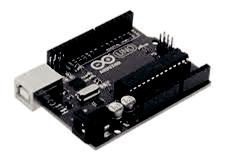
\includegraphics[width=0.5\textwidth]{image14.jpeg}

Cette partie s'intéresse

maintenant à la génération de la consigne de

position à appliquer à chacun de ces pieds via une

carte de commande. \textbf{Figure 14} -- Carte Arduino Uno

On dispose d'une carte Arduino Uno qui peut être programmée dans
différents langages. \textbf{On se} \textbf{limitera à l'utilisation du
langage de programmation Python pour l'étude proposée}.

Le calculateur (la carte Arduino dans notre cas), qui contrôle le
mouvement des trois vérins électriques, génère, pour chaque vérin, un
signal de consigne rapide (vitesse maximale du moteur) ou lent (un
dixième de la vitesse maximale du moteur) en fonction de l'avance de
celui-ci. Dans une première phase, il génère une consigne dite « rapide
» jusqu'à atteindre une distance de 10 mm entre la tige du vérin et le
sol. Le système de commande délivre alors une consigne dite « lente »
afin de limiter les contraintes lors du contact entre chaque vérin et le
sol. Lors de cette deuxième phase (consigne « lente »), un
asservissement en position de chaque vérin permet de maintenir le
châssis du SEIS en position horizontale par rapport au sol.

On note pour la suite de l'étude (\textbf{figure 15}) :

\begin{itemize}
\item
  \textbf{distance} : la variable, de type float, correspondant à la
  distance mesurée entre le sol et le capteur donnée en cm ;
\item
  \textbf{distance\_verin} : la variable, de type float, correspondant à
  la distance entre le capteur et l'extrémité de la tige du vérin donnée
  en cm ;
\item
  \textbf{rapide} et \textbf{lente} : variable globale avec des valeurs
  prédéfinies (correspond aux consignes
\end{itemize}

de la commande du vérin électrique : vitesse rapide, vitesse lente).

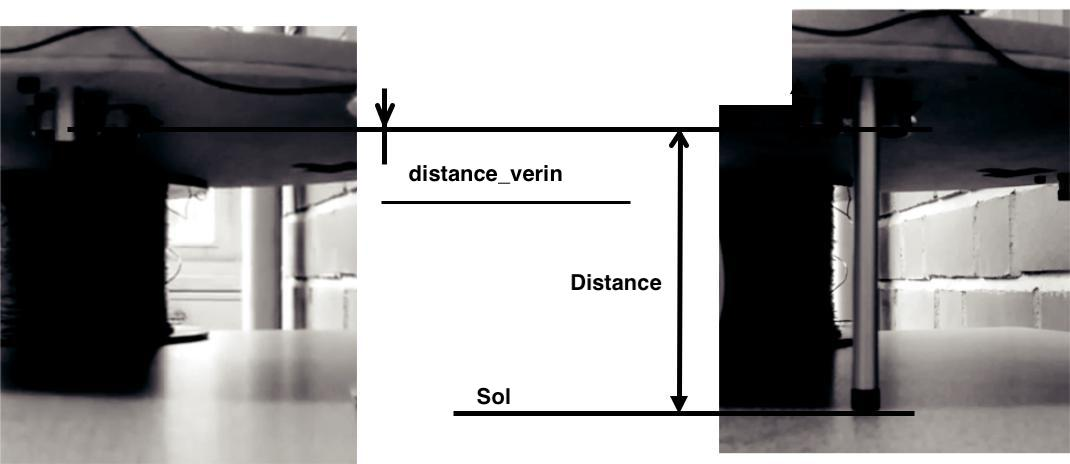
\includegraphics[width=4.95347in,height=2.15000in]{image15.jpeg}

capteur

ultrasons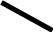
\includegraphics[width=0.24722in,height=0.14861in]{image16.jpeg}

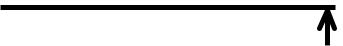
\includegraphics[width=1.58958in,height=0.21111in]{image17.jpeg}
distance\_vérin

distance

sol

\textbf{Figure 15} -- Sortie du vérin 1

\textbf{Q26.} Écrire une fonction
\textbf{consigne(distance,distance\_verin)} qui calcule l'écart entre la
tige du vérin et le sol et qui retourne la consigne \textbf{rapide} si
cet écart est supérieur à 10 mm ou

la consigne \textbf{lente} sinon.

Le module SEIS est équipé de trois
capteurs de positions, à ultrasons, associés à chaque vérin électrique.
Chaque capteur est constitué d'un émetteur et d'un récepteur à
ultrasons. Le principe de mesure des capteurs à ultrasons utilisés est
donné ci-dessous et illustré sur la \textbf{figure 16}.

Pour déclencher une mesure, il faut présenter une impulsion « High » (5
V) d'au moins 10 $\mu s$ sur l'entrée « Trig » du capteur (sortie de la carte
Arduino). L'émetteur à ultrasons délivre alors une série de 8 impulsions
ultrasoniques à 40 kHz, puis il attend le signal réfléchi. Lorsque
celui-ci est détecté par le récepteur à ultrasons, le capteur impose un
signal « High » sur la sortie « Echo » (entrée de la

carte Arduino) dont la durée, tc, est proportionnelle à la distance
mesurée. La distance est obtenue en

multipliant la durée du signal tc en seconde par le coefficient constant
17 150 pour obtenir la valeur de la distance en cm.

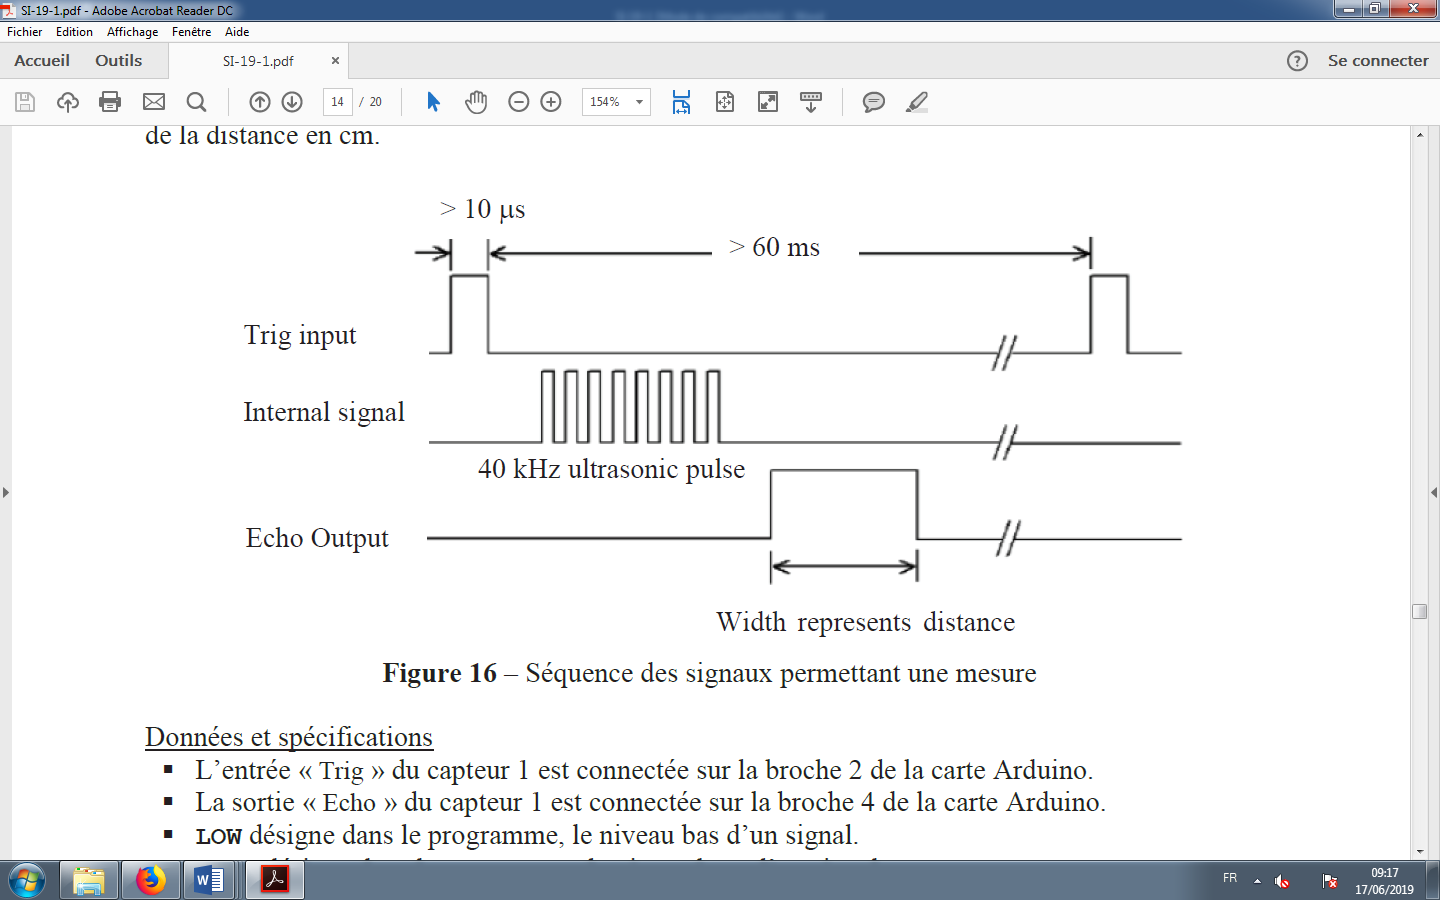
\includegraphics[width=4.56000in,height=2.47917in]{image18.png}